\documentclass[t, pdftex]{beamer}
\usetheme[]{Cockrell}
%\usetheme[dept=Aerospace\ Engineering\ and\ Engineering\ Mechanics]{cockrell}
%\usetheme[dept=Biomedical\ Engineering]{cockrell}
%\usetheme[dept=Chemical\ Engineering]{cockrell}
%\usetheme[dept=Civil,\ Architectural\ and\ Environmental\ Engineering]{cockrell}
%\usetheme[dept=Electrical\ and\ Computer\ Engineering]{cockrell}
%\usetheme[dept=Mechanical\ Engineering]{cockrell}
%\usetheme[dept=Materials\ Science\ and\ Engineering]{cockrell}
%\usetheme[dept=Petroleum\ and\ Geosystems\ Engineering]{cockrell}

% Packages
%\usepackage{etex}
%\usepackage[bigfiles]{media9}
%\graphicspath{{./figs/}}

%Enable cancelto in math
\usepackage{cancel}
\usepackage[]{algorithm2e}
\usepackage{mathtools}
\usepackage{pgfgantt}
\usepackage[version=3]{mhchem} % Package for chemical equation typesetting \ce{}
\usepackage{siunitx} % Provides the \SI{}{} and \si{}
\renewcommand{\CancelColor}{\color{utorange}}

%Add bibliography file location for citiation
\bibliography{example.bib}


\title{A Hi2Low Method for Improving\\ CRUD Predictions}
\subtitle{Using Copula and Gradient Boosted Regression Trees}
\author{William Gurecky}
\institute{PhD Proposal}
\date{\today}


\begin{document}

% =========================================================================== %
\titleframe
\frame{\frametitle{Outline}\tableofcontents}

% =========================================================================== %
\section{Hi2Low Approach}
\begin{frame}
    \frametitle{CFD informed surrogate model to improve CRUD growth}
    \begin{itemize}
    \item Construct a scale bridging model which utilizes a suite of pre-computed CFD solutions to improve CRUD predictions given on the CTF grid. 
    \item CTF estimates mean TH conditions everywhere in the core at a low spatial resolution.  The surrogate provides higher order moments about the mean.
    \end{itemize}
    \begin{block}{Rod Surface Field}
        \[ 
        F(\mathbf z) = \underbrace{\mu(\mathbf{z})}_\text{CTF} + \underbrace{\varepsilon({\mathbf z, \mathbf p(\mathbf z)})}_\text{CFD Informed} + b(\mathbf{z})
        \]
    \end{block}
    Treat $\varepsilon$ as a random field.  $\varepsilon(\cdot)$ is a CFD informed model. $\mathbf z$ are spatial coordinates. $\mathbf p$ are a set of auxiliary predictors. \\
    $b$ is bias ($\mu_{CTF} - \mu_{CFD}$) \\
    $\mu$ are spatially averaged over a CTF patch
\end{frame}

% =========================================================================== %
\begin{frame}\frametitle{Objectives}
\begin{itemize}
\item Account for fine scale flow features unresolved by CTF on the growth of CRUD and boron hideout.
\item Proposed Hi2Low Approach:
\begin{itemize}
	\item Forgo attempting to capture spatial distributions of temperature, boundary heat flux and TKE on rod surface. 
	\item Instead, track joint probability density $f(T, TKE, q'')$ tallied over coarse CTF patches.
\end{itemize}
	\item Predict likelihood of temperatures in excess of saturation occurring in coincidence with low local turbulent kinetic energy.
	\item Capture the dependence between surface temperature and turbulent kinetic energy.
\end{itemize}
\end{frame}

% =========================================================================== %
\begin{frame}[shrink=10]
    \frametitle{Chalk River Unidentified Deposit (CRUD)}
    CRUD forms a porous layer on the surface of fuel rods.
    \begin{itemize}
    \item Preferentially deposited where temperature is high - near or above saturation point - and where local shear stresses on the rod are low.
	\item CRUD induced local corrosion (CILC).
    \item CRUD induced power shift (CIPS). In industry known as axial offset anomaly (AOA).
    \begin{itemize} 
    	\item CRUD and tends to uptake and retain boron from the coolant.
    	\item \ce{Li^+} + \ce{B(OH)_3}   $\rightarrow$ \ce{LiBO_2} + \ce{H^+} + \ce{H_2O} .
    \end{itemize}
    \item CASL developed CRUD simulation packages: MAMBA \& Mongoose
    \end{itemize}
%\begin{figure}[!htbp]
%\centering
%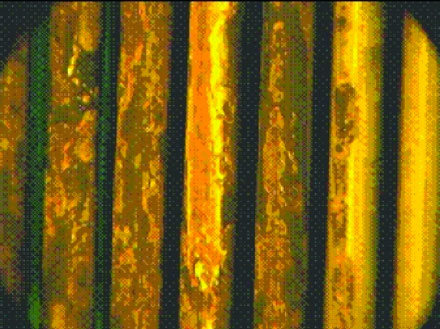
\includegraphics[width=4cm]{figs/crud-crud.jpg}
%\caption{CRUD on fuel rods.}
%\label{log_closed}
%\end{figure}
%
    \begin{figure}
        \centering
        \begin{minipage}{.7\textwidth}
            \centering
            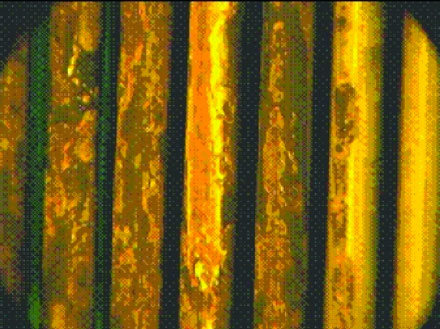
\includegraphics[width=6cm]{figs/crud-crud.jpg}
        \end{minipage}%
        \begin{minipage}{.4\textwidth}
            \centering
            \includegraphics[width=6cm]{figs/crud_flake_ex.png}
        \end{minipage}
    \end{figure}
\end{frame}

% =========================================================================== %
\section{Background}
\begin{frame}
    \frametitle{Chalk River Unidentified Deposit (CRUD)}
    \begin{figure}
        \centering
        \begin{minipage}{.5\textwidth}
            \centering
            \includegraphics[width=6cm]{figs/ao_mpact_ctf.png}
            \caption{Core averaged \% axial offset. [CASL-I-2015-0318-000]}
        \end{minipage}%
        \begin{minipage}{.5\textwidth}
            \centering
            \includegraphics[width=6cm]{figs/core_b10_mpact_ctf.png}
            \caption{VERA WBNP1 Cycle 7 CRUD \ce{^{10}B}. 16.08 $[MWD/MTU]$}
        \end{minipage}
    \end{figure}
\end{frame}

% =========================================================================== %
\begin{frame}[shrink=20]
    \frametitle{Coupled CFD/CRUD Calculation}
    \begin{itemize}
    \item CFD/CRUD coupling is useful for single-pin or single-assembly CRUD estimates.
    \item High fidelity CFD/CRUD simulations are too numerically costly for full core simulation.
    \end{itemize}
        \begin{figure}[!htbp]
\centering
\includegraphics[width=14cm]{figs/combo_180x.png}
\label{log_closed}
    \end{figure}
\end{frame}

% =========================================================================== %
\begin{frame}[shrink=10]
    \frametitle{Prior Art: HTC Remapping Hi2Low Procedure}
\begin{columns}
\begin{column}{0.5\textwidth}
   \begin{itemize}
   \item Salko et. al (2017) developed a Hi2Low procedure based on mapping and re-scaling CFD results onto an intermediate reconstruction grid upon which CRUD is grown.
   \item The single phase heat transfer coefficient (HTC) and TKE surface fields are mapped.
   \item An iterative method is used to converge on the correct pin surface temperature given HTC and the boundary heat flux provided by CTF.
   \end{itemize}
\end{column}
\begin{column}{0.5\textwidth}  %%<--- here
    \begin{center}
    \begin{figure}
     \includegraphics[width=5cm]{figs/cfd_ctf_multi_grid.png}
     \caption{TKE remapping procedure.}      
    \end{figure}
     \end{center}
\end{column}
\end{columns}
\end{frame}

% =========================================================================== %
\begin{frame}
    \frametitle{Prior Art: HTC Remapping Hi2Low Procedure}
    \begin{figure}[!htbp]
\centering
\begin{minipage}{.5\textwidth}
  %
  \includegraphics[width=5cm]{figs/ctf_crud_orig.png}
\caption{CRUD growth on the rod surface prior to HTC and TKE field remapping.}
\label{fig:crud_pre_map}
\end{minipage}%
\begin{minipage}{.5\textwidth}
  %
  \includegraphics[width=5cm]{figs/ctf_crud_reconstructed.png}
\caption{CRUD growth on the rod surface post HTC and TKE field remapping.}
\label{fig:crud_post_map}
\end{minipage}
\end{figure}
\end{frame}

% =========================================================================== %
\begin{frame}
Differences between CTF and CFD meshes for a single pin.
\begin{figure}
        \centering
        \begin{minipage}{.4\textwidth}
            \centering
            \includegraphics[width=3cm]{figs/cfd_ctf_mesh_v.png}
        \end{minipage}%
        \begin{minipage}{.4\textwidth}
            \centering
            \includegraphics[width=2cm]{figs/ctf_mesh_v.png}
        \end{minipage}
\end{figure}
\end{frame}

% =========================================================================== %
\begin{frame}
\begin{figure}[!htbp]
\centering
\includegraphics[width=10.88cm]{figs/ctf_patch_ex3.png}
\label{model_overview}
\end{figure}
\end{frame}

% =========================================================================== %
\begin{frame}
On a single coarse CTF patch:
\begin{figure}[!htbp]
\centering
\includegraphics[width=11cm]{figs/model_relations.png}
\label{model_overview}
\end{figure}
\end{frame}

% =========================================================================== %
\section{Capturing Dependence between Random Variables}
\begin{frame}
\frametitle{Capturing Dependence - Sklar's Theorem}
\begin{itemize}
\item Given joint CDF: $H$, w/ cumulative margins: $F(x)=P[X < x] = \int_{-\infty}^{x}f(t)dt$
\[
H(x,y) = C(F(x), F(y))
\]
\[
c(u, v) = \frac{\partial^2 C(u, v)}{\partial u \partial v};\ u=F(x), v=F(y)
\]
\item  The copula PDF, $c(\cdot)$ is describes dependence between two random variables.
\item  Has uniform marginal density distributions \cite{Nelsen2006}.
\item  Defined on the unit square $[0, 1]^2$ (in the bivariate case)
\item  Any joint PDF, $h(\cdot)$ can be decomposed as: \\
\[
h(x, y) = c(F(x), F(y)|\theta_c)f(x|\theta_x)f(y|\theta_y)
\]
Where $\theta_c$ and $\theta_{x,y}$ are free copula and marginal model parameters respectively.
\end{itemize}
\end{frame}


% =========================================================================== %
\begin{frame}
\frametitle{Specifying Copula Parameters}
\begin{itemize}
\item For the case of Archimedean copula, Kendall's tau, $\rho_\tau$ is
related to the copula's shape parameter by:
\[
\rho_\tau = 1 + 4 \int_0^1 \frac{\varphi(\theta_c,t)}{\varphi'(\theta_c, t)}dt
\]
Where $\varphi(\theta_c, t)$ is the copula's generator function and $\varphi'$ is the first derivative of the generator function with respect to $t$.
\item  If we restrict ourselves to the class of  Archimedean copula we only need $\rho_\tau$ and the copula type, $\Theta_c$ (gumbel, frank, clayton, ect.) to approximately specify the dependence structure between the temperature and turbulent kinetic energy residual distributions in each CTF patch.
\item Must associate each CTF patch with a copula family (categorical response) and Kendall's tau (real-valued).
\end{itemize}
\end{frame}

% =========================================================================== %
\section{Gradient Boosted Tree Regression}
\begin{frame}
\frametitle{Gradient Boosted Regression Model}
Goal: Build regression model $G(\mathbf p)$, that returns $\rho_\tau$, the copula type $\Theta_c$ and the marginal T and TKE distribution parameters $\theta_{x,y}$ given some predictors $\mathbf p$.
\begin{itemize}
\item The predictors identify a CTF patch.  For the $i^{th}$ CTF patch let: $p_i = \{ \Delta z_i, T_i,  TKE_i, q_i^{''} \}_{ctf}$.  Where $\Delta z$ is axial distance to nearest upstream spacer grid.
\item $\Theta_c$ is a categorical response.
\item $\rho_\tau$ is real valued.
\item $\theta_{x,y}$ are the margin parameters.  These are also real valued.
\item Upon evaluation $ \{\Theta_c, \rho_\tau, \theta_{x,y}\}_i \leftarrow G(p_i)$
\begin{itemize}
\item Allows recovery of joint distribution on $i^{th}$ CTF patch:
\[
h_i(x, y) = c(F(x), F(y)|\rho_{\tau_i}) f(x|\theta_{x_i}) f(y|\theta_{y_i})
\]
\end{itemize}
\end{itemize}
\end{frame}

% =========================================================================== %
\begin{frame}
\frametitle{Non-Parametric Representation of the Margins}
\begin{itemize}
\item The proposed method uses a non-parametric representation of the margins.
\begin{itemize}
	\item In the parametric approach we would predict the ``shape'' parameters $\theta_{x}(\mathbf{p})$.
	\item In the non-parametric approach $\theta_x$ is replaced by a vector of conditional quantiles, $\mathbf Q_\tau (\mathbf p)$.
\end{itemize}
\item  Each conditional quantile (ex: Median of the temperature distribution) is a function of $\mathbf p$. A gradient boosted regression tree is fit to each quantile independently.
\end{itemize}
\end{frame}

% =========================================================================== %
\begin{frame}[shrink=20]
\frametitle{Obtaining the Margins}
\begin{itemize}
\item $Q_\tau = F^{-1}(\tau); $ where $\ F(y)=P[Y \leq y]$ is a CDF.
\item $\tau \in [0, 1]$

\item The quantile loss function is given by:
\[
\rho_\tau(u) = u \cdot (\tau - \mathbb{I}_{(u < 0)});\ u=Y - Q_\tau
\]
\item The quantile loss function is utilized as the general loss function, $L$, in the gradient boosting algorithm.  The derivative of the loss function is provided in the image below.
\end{itemize}
\begin{figure}
        \centering
        \begin{minipage}{.5\textwidth}
            \centering
            \includegraphics[width=5cm]{figs/q_loss.png}
        \end{minipage}%
        \begin{minipage}{.5\textwidth}
            \centering
            \includegraphics[width=10cm]{figs/1d_boosted_regression_quantile_ex.png}
        \end{minipage}
\end{figure}
\end{frame}

% =========================================================================== %
\begin{frame}[shrink=20]
\frametitle{Gradient Boosting Algorithm}

The generalized gradient boosting algorithm was developed by Friedman (1999).
Let $y$ be some quantile of interest $Q_{\tau_{y_i}}$.
\begin{algorithm}[H]
\KwData{ (1) Training set $\{(p_i, y_i)\}_{i=1}^n$. (2) Differentiable loss function $L(y, F(p))$. (3) Number of iterations ${{M}}$.
Initialize model with a constant value:
$F_0(p) = \underset{\gamma}{\arg\min} \sum_{i=1}^n L(y_i, \gamma).$}

\For{${{m}} = 1$ to ${{M}}$}{
Compute the pseudo-residuals:

\For{$i=1,\ldots,n $}{
$r_{im} = -\frac{\partial L(y_i, F_{m-1}(p_i))}{\partial F_{m-1}(p_i)}$
}

Fit a weak learner $h_m(p)$ to pseudo-residuals, $r_{m}$: Training data set is $\{(p_i, r_{im})\}_{i=1}^n$ \;

Compute multiplier $\gamma_m$ :
$\gamma_m = \underset{\gamma}{\operatorname{arg\,min}} \sum_{i=1}^n L\left(y_i, F_{m-1}(p_i) + \gamma h_m(p_i)\right)$\;
Update the model:
$F_m(p) = F_{m-1}(p) + \nu \gamma_m h_m(p).$
}
Output $F_M(p).$
\end{algorithm}
Where $\nu$ is a tunable constant in $[0, 1]$ called the learning rate.
\end{frame}

% =========================================================================== %
\begin{frame}[shrink=20]
\frametitle{Single Statepoint Hi2Low Procedure}
Up front:
\begin{itemize}
\item (1) - De-trend CFD temperature, $q''$, and TKE surface fields.	
\item (2) - Compute residual (CFD-CTF) distribution statistics on each CTF patch.
	\begin{itemize}
	\item  Fit trial copula to joint distributions via maximum likelihood. 
	\item  Obtain empirical $\rho_\tau$ and select the best-fitting copula, as judged by AIC (see Appendix A). 
	\end{itemize}
\item (3) - Fit gradient boosted regression/classification models.  Builds a relationship between the local-average CTF TH conditions and copula and margin parameters.
\end{itemize}
At run time:
\begin{itemize}
\item (4) - Execute a CTF simulation.
\item (5) - For each CTF patch:
\begin{itemize}
\item Evaluate the regression model(s) in the CTF patch.
	\begin{itemize}
	\item  Obtain copula family, $\hat \Theta_c$.
	\item  Obtain conditional quantiles $\hat Q_\tau(T)$ and $\hat Q_\tau(TKE)$ 
	\item  Reconstruct $f(T)$, $f(TKE)$ margins. Assume $q''$ is uniform over a CTF patch.
	\end{itemize}
\item Reconstruct the joint density function, $f(T, TKE, q'')$, from the predicted conditional quantiles, the predicted copula family, $\hat \Theta_c$, and $\hat \rho_\tau$.  
\item Draw $N$ TH samples from the predicted joint $f(T, TKE, q'')$ distribution.  
\item Use $N$ TH samples as boundary conditions to $N$ independent CRUD (MAMBA1D) simulations.
\item Integrate CRUD results over the CTF patch.
\item Pass the patch-integrated CRUD results to the CTF grid.
\end{itemize}
\end{itemize}
\end{frame}

% =========================================================================== %
\begin{frame}
\frametitle{Single Statepoint Hi2Low Procedure}
The $i^{th}$ CRUD sample drawn from CTF patch, $j$:
\begin{figure}[!htbp]
\centering
\includegraphics[width=9cm]{figs/crud_samples.png}
\label{model_overview}
\end{figure}
\begin{itemize}
\item Samples are drawn with weight $w_i=A_p/N$ where $A_p$ is the CTF patch area and $N$ is the total number of samples/patch.
\item TH boundary conditions are held fixed throughout the duration of the CRUD simulation step with timestep size $\Delta t$.
\end{itemize}
\end{frame}

% =========================================================================== %
\begin{frame}[shrink=20]
\frametitle{Generating Synthetic CFD Data}
\begin{itemize}
\item Cheaply generates CFD-like data sets with user-provided residual model.
\item Applies tailored noise on top of CTF result.
\begin{itemize}
	\item Complete control over margins and copula. 
\end{itemize}
\item Aids in verification of regression model results. 
\end{itemize}
\begin{figure}
        \centering
        \begin{minipage}{.5\textwidth}
            \centering
            \includegraphics[width=7.5cm]{figs/pinTempOut.png}
            \caption{Synthetic CFD Temperature $[K]$ distribution vs. axial position.}
        \end{minipage}%
        \begin{minipage}{.5\textwidth}
            \centering
            \includegraphics[width=7.5cm]{figs/pinTkeOut.png}
            \caption{Synthetic CFD TKE  $[J/Kg]$ distribution vs. axial position.}
        \end{minipage}
    \end{figure}
\end{frame}

% =========================================================================== %
\section{Results}
\begin{frame}\frametitle{Single Pin CTF/MAMBA1D Results}
    \begin{figure}
        \centering
        \begin{minipage}{.5\textwidth}
            \centering
            \includegraphics[width=4.3cm]{figs/single_pin_ctf_conds.png}
            \caption{Single pin CTF inputs.}
        \end{minipage}%
        \begin{minipage}{.5\textwidth}
            \centering
            \includegraphics[width=6cm]{figs/b10_ctf_out.png}
            \caption{CTF/MAMBA1D Boron Hideout Mass Density $[g/cm^2]$}
        \end{minipage}
    \end{figure}
CRUD result at 100$[days]$.
\end{frame}

% =========================================================================== %
\begin{frame}\frametitle{Single Pin CTF/MAMBA1D Results}
    \begin{figure}
        \centering
        \begin{minipage}{.5\textwidth}
            \centering
            \includegraphics[width=6cm]{figs/crud_ctf_out.png}
            \caption{CTF/MAMBA1D CRUD Mass Density $[g/cm^2]$}
        \end{minipage}%
        \begin{minipage}{.5\textwidth}
            \centering
            \includegraphics[width=6cm]{figs/b10_ctf_out.png}
            \caption{CTF/MAMBA1D Boron Hideout Mass Density $[g/cm^2]$}
        \end{minipage}
    \end{figure}
CRUD result at 100$[days]$.
\end{frame}

% =========================================================================== %
\begin{frame}\frametitle{Single Pin Hi2Low Results}
    \begin{figure}
        \centering
        \begin{minipage}{.5\textwidth}
            \centering
            \includegraphics[width=6cm]{figs/tke_cfd_out.png}
            \caption{Synthetic CFD TKE distribution (Blue).}
        \end{minipage}%
        \begin{minipage}{.5\textwidth}
            \centering
            \includegraphics[width=6cm]{figs/tke_model_out.png}
            \caption{Hi2Low TKE prediction (Blue).}
        \end{minipage}
    \end{figure}
$68^{th}, 95^{th}, 98^{th}$ percentiles shown.
CTF baseline shown in green.
\end{frame}

% =========================================================================== %
\begin{frame}\frametitle{Single Pin Hi2Low Results}
    \begin{figure}
        \centering
        \begin{minipage}{.5\textwidth}
            \centering
            \includegraphics[width=6cm]{figs/twall_cfd_out.png}
            \caption{Synthetic CFD temperature distribution (Blue).}
        \end{minipage}%
        \begin{minipage}{.5\textwidth}
            \centering
            \includegraphics[width=6cm]{figs/twall_model_out.png}
            \caption{Hi2Low temperature prediction (Blue).}
        \end{minipage}
    \end{figure}
$68^{th}, 95^{th}, 98^{th}$ percentiles shown.
Area weighted average in dark blue.  CTF baseline shown in green.  CRUD result at 100$[days]$.
\end{frame}

% =========================================================================== %
\begin{frame}\frametitle{Single Pin Hi2Low Results}
    \begin{figure}
        \centering
        \begin{minipage}{.5\textwidth}
            \centering
            \includegraphics[width=6cm]{figs/b10_cfd_out.png}
            \caption{Sythetic CFD Boron Hideout Mass Density $[g/cm^2]$}
        \end{minipage}%
        \begin{minipage}{.5\textwidth}
            \centering
            \includegraphics[width=6cm]{figs/b10_model_out.png}
            \caption{Hi2Low Boron Hideout Mass Density $[g/cm^2]$}
        \end{minipage}
    \end{figure}
$68^{th}, 95^{th}, 98^{th}$ percentiles shown.
Area weighted average in dark blue.  CTF baseline shown in green.  CRUD result at 100$[days]$.
\end{frame}

% =========================================================================== %
\begin{frame}\frametitle{Single Pin Hi2Low Results}
    \begin{figure}
        \centering
        \begin{minipage}{.5\textwidth}
            \centering
            \includegraphics[width=6cm]{figs/crud_cfd_out.png}
            \caption{Sythetic CFD Hi2Low CRUD Mass Density $[g/cm^2]$}
        \end{minipage}%
        \begin{minipage}{.5\textwidth}
            \centering
            \includegraphics[width=6cm]{figs/crud_model_out.png}
            \caption{Hi2Low CRUD Mass Density $[g/cm^2]$}
        \end{minipage}
    \end{figure}
$68^{th}, 95^{th}, 98^{th}$ percentiles shown.
Area weighted average in dark blue.  CTF baseline shown in green.  CRUD result at 100$[days]$.
\end{frame}



% =========================================================================== %
\begin{frame}\frametitle{Single Pin CTF Results}
\begin{table}[h!]
\begin{center}
\begin{tabular}{|c|c|c|c|}
\hline 
 QOI  &   CTF	&  CFD (Synthetic)	& Hi2Low Model \\ \hline
Total Boron Mass [g]& 0.00587	&  0.00496	& 0.00631 \\
Total CRUD Mass [g]	& 8.788	&  7.155 & 9.042	\\
\hline
\end{tabular}
\caption{Single pin CRUD result summary.}
\label{tab:crud_res}
\end{center}
\end{table}
\begin{itemize}
\item CRUD result at 100$[days]$.  
\item CFD data detrended via moving average.  In this case the residual CFD$-$CTF distributions are stationary about 0.
\end{itemize}
\end{frame}

% =========================================================================== %
\begin{frame}\frametitle{TKE Gradient Boosted Quantile Regression Results}
    \begin{figure}
        \centering
        \begin{minipage}{.5\textwidth}
            \centering
            \includegraphics[width=6cm]{figs/tke_quantile_model_out.png}
            \caption{Hi2Low predicted TKE residual quantiles $[J/kg]$ vs Axial position $[m]$.}
        \end{minipage}%
        \begin{minipage}{.5\textwidth}
            \centering
            \includegraphics[width=6cm]{figs/qq_plot_tke_69.png}
            \caption{Q-Q Plot comparing gradient boosted quantiles vs. synthetic CFD data. $z=2.59[m]$}
        \end{minipage}
    \end{figure}
Quantiles used in TKE residual reconstruction: $\tau_{TKE}=\{0, 0.01, 0.05, 0.15, 0.3, 0.5, 0.7, 1\}$
\end{frame}

% =========================================================================== %
\begin{frame}\frametitle{TKE Gradient Boosted Quantile Regression Results}
    \begin{figure}
        \centering
        \begin{minipage}{.5\textwidth}
            \centering
            \includegraphics[width=6cm]{figs/tke_quantile_model_out.png}
            \caption{Hi2Low predicted TKE residual quantiles $[J/kg]$ vs Axial position $[m]$.}
        \end{minipage}%
        \begin{minipage}{.5\textwidth}
            \centering
            \includegraphics[width=6cm]{figs/qq_plot_tke_76.png}
            \caption{Q-Q Plot comparing gradient boosted quantiles vs. synthetic CFD data. $z=2.84[m]$}
        \end{minipage}
    \end{figure}
Quantiles used in TKE residual reconstruction: $\tau_{TKE}=\{0, 0.01, 0.05, 0.15, 0.3, 0.5, 0.7, 1\}$
\end{frame}

% =========================================================================== %
\begin{frame}\frametitle{Temperature Gradient Boosted Quantile Regression Results}
    \begin{figure}
        \centering
        \begin{minipage}{.5\textwidth}
            \centering
            \includegraphics[width=6cm]{figs/t_quantile_model_out.png}
            \caption{Hi2Low predicted temperature residual quantiles $[K]$ vs Axial position $[m]$.}
        \end{minipage}%
        \begin{minipage}{.5\textwidth}
            \centering
            \includegraphics[width=6cm]{figs/qq_plot_t_69.png}
            \caption{Q-Q Plot comparing gradient boosted quantiles vs. synthetic CFD data. $z=2.59[m]$}
        \end{minipage}
    \end{figure}
Quantiles used in temperature residual reconstruction: $\tau_{T}=\{0, 0.1, 0.3, 0.5, 0.7, 0.85, 0.9 0.95, 0.99, 1\}$
\end{frame}

% =========================================================================== %
\begin{frame}\frametitle{Temperature Gradient Boosted Quantile Regression Results}
    \begin{figure}
        \centering
        \begin{minipage}{.5\textwidth}
            \centering
            \includegraphics[width=6cm]{figs/t_quantile_model_out.png}
            \caption{Hi2Low predicted temperature residual quantiles $[K]$ vs Axial position $[m]$.}
        \end{minipage}%
        \begin{minipage}{.5\textwidth}
            \centering
            \includegraphics[width=6cm]{figs/qq_plot_t_76.png}
            \caption{Q-Q Plot comparing gradient boosted quantiles vs. synthetic CFD data. $z=2.84[m]$}
        \end{minipage}
    \end{figure}
Quantiles used in temperature residual reconstruction: $\tau_{T}=\{0, 0.1, 0.3, 0.5, 0.7, 0.85, 0.9 0.95, 0.99, 1\}$
\end{frame}

% =========================================================================== %
\begin{frame}\frametitle{GBRT Output - Copula Parameters}
\begin{figure}[!htbp]
\centering
\includegraphics[width=8cm]{figs/ktau_plot.png}
\label{model_overview}
\end{figure}
\begin{itemize}
\item Red - Frank Copula
\item Green - Gaussian Copula
\item Blue - Clayton Copula
\end{itemize}
\end{frame}



% =========================================================================== %
\section{Future Work}
\begin{frame}\frametitle{Future Work}
\begin{itemize}
\item Multi-state point execution.
\begin{itemize}
	\item Grow CRUD at updated TH conditions.
	\item Account for previous CRUD history, as the CRUD layer provides TH feedback.
	\item Aggregate the ensemble of CRUD predictions on each CTF patch.
	\item Propagate CRUD ensemble prediction errors forward in time.
\end{itemize}
\end{itemize}
\begin{figure}[!htbp]
\centering
\includegraphics[width=7cm]{figs/crud_samples_dt.png}
\label{model_overview}
\end{figure}
\begin{itemize}
\item Quantify uncertainty in each quantity predicted by the GBRT.
\item Propagate uncertainties through the MAMBA runs.
\end{itemize}
\end{frame}

% =========================================================================== %
\begin{frame}
\frametitle{Conclusion}
\begin{itemize}
\item The proposed technique does not try to provide a detailed spatial distribution
of the temperature, TKE, and CRUD on the rods' surface.
\item The proposed approach seeks to predict detailed joint frequency distributions on each CTF patch.
\item Treatment of the bias term is important wrt. Hi2Low CRUD results.
\item Time stepping scheme must account for the ensemble approach to CRUD growth.
\item Future work will focus on uncertainty quantification.
\end{itemize}
\end{frame}

% =========================================================================== %
\begin{frame}[shrink=50]
\frametitle{Project Schedule: Year 1}
\begin{ganttchart}[
        inline,
        x unit=1.5cm,
        y unit title =0.8cm,
        y unit chart=0.8cm,
        hgrid,
        vgrid,
        time slot format=isodate,
        compress calendar
    ]{2016-06-01}{2017-07-30}
    \gantttitlecalendar*[compress calendar, time slot format=isodate]{2016-06-01}{2017-07-30}{year, month=shortname} \\
    \gantttitlelist{1,...,14}{1} \\
%%%%%%% Phase 1
\ganttgroup{Proposal Era}{2016-06-01}{2017-06-30} \\  %elem0
\ganttbar{Lit. Review}{2016-06-01}{2016-11-01} \\  %elem1
\ganttbar{CFD Post Proc. Dev.}{2016-06-01}{2016-08-20} \\  %elem2
\ganttlinkedbar{CTF vs CFD}{2016-08-20}{2016-10-30} \ganttnewline  %elem3
\ganttbar{MAMBA Sensitivity}{2016-08-01}{2016-09-30} \ganttnewline  %elem4
\ganttbar{Copula Model Dev.}{2016-10-01}{2017-01-10}  \\  %elem5
\ganttbar{Synthetic Data Gen}{2016-12-01}{2017-01-30} \\  %elem6
\ganttlinkedbar{GBRT Model Dev.}{2016-12-01}{2017-03-30}  \\  %elem7
\ganttlinkedbar{Link Models w/ CRUD Sim.}{2017-03-01}{2017-06-30}  \\  %elem8
\ganttbar{Write Proposal}{2017-04-01}{2017-06-30}  %elem9
\ganttmilestone{Proposal}{2017-06-30} \ganttnewline  %elem10
%%%%%%%% Extra Task Linkages
\ganttlink[link mid=0.2]{elem2}{elem4}
\end{ganttchart}
\end{frame}

% =========================================================================== %
\begin{frame}[shrink=50]
\frametitle{Project Schedule: Year 2}
\begin{ganttchart}[
        inline,
        x unit=2.5cm,
        y unit title =0.8cm,
        y unit chart=0.8cm,
        hgrid,
        vgrid,
        time slot format=isodate,
        compress calendar
    ]{2017-06-01}{2018-01-30}
    \gantttitlecalendar*[compress calendar, time slot format=isodate]{2017-06-01}{2018-01-30}{year, month=shortname} \\
    \gantttitlelist{13,...,20}{1} \\
%%%%%%% Phase 2
\ganttbar{ }{2017-06-01}{2017-06-30}  %elem0
\ganttmilestone{Proposal}{2017-06-30} \ganttnewline  %elem1
\ganttgroup{Dissertation Era}{2017-07-1}{2018-01-01} \\  %elem2
\ganttbar{Time Stepping}{2017-07-01}{2017-08-01} \ganttnewline  %elem3
\ganttlinkedbar{Uncert. Prop}{2017-08-01}{2017-09-01} \ganttnewline  %elem4
\ganttbar{Methods Refinement}{2017-08-01}{2017-10-01} \ganttnewline  %elem5
\ganttbar{Final CFD Runs}{2017-10-01}{2017-11-01} \ganttnewline  %elem6
\ganttbar{Write Dissertation}{2017-10-01}{2017-12-15}  %elem7
\ganttmilestone{Defense}{2017-12-15} \ganttnewline  %elem8
\ganttlinkedbar{Final Revisions}{2018-01-01}{2018-01-30}  \ganttnewline  %elem9
\ganttmilestone{Project Conclusion}{2018-01-30} \ganttnewline  %elem10
%%%%%%%% Extra Task Linkages
\end{ganttchart}
\end{frame}

% =========================================================================== %
\begin{frame}
\frametitle{Questions?}
\end{frame}

% =========================================================================== %
\begin{frame}[shrink=10]
\frametitle{Classification and Regression Tree (CART) - Weak Learner}
Each weak learner in the ensemble is a binary tree that partitions the input space based on "best-first" splits.  
\begin{itemize}
\item classification - find the split that minimizes: $-\sum_j\sum_i f_{ij} ln(f_{ij})$, where $f_{ij}$ is the fraction of class label $i$ in the region $j$.
\item Least squares regression - find the split that minimizes: $\sum_j\sum_i(y_i - \hat y_{j})^2$
\end{itemize}

\begin{figure}[!htbp]
\centering
\includegraphics[width=7cm]{figs/cart.png}
\label{model_overview}
\end{figure}
\end{frame}

% =========================================================================== %
\begin{frame}
\frametitle{GBRT - Weak Learners Fit to Pseudo Residuals}
Weak learners are fit the the pseudo-residuals (derivative of the loss function): 
\[
\frac{\partial L(y_i, F(p_i))}{\partial F(p_i)}
\]
if $L_i=0.5(y_i-F(p_i))^2$ then $L' = F(p_i)-y_i$.  
\begin{figure}[!htbp]
\centering
\includegraphics[width=9cm]{figs/pseudo_resids.png}
\label{model_overview}
\end{figure}
Source: Peter Prettenhofer, PyData (2014).
\end{frame}

% =========================================================================== %
\begin{frame}
\frametitle{GBRT - Ensemble of weak learners}

\begin{figure}[!htbp]
\centering
\includegraphics[width=8.5cm]{figs/1d_boosted_regression_ex.png}
\label{model_overview}
\end{figure}
\end{frame}

% =========================================================================== %
\begin{frame}[shrink=10]
\frametitle{Overfitting Detection and Prevention}
\begin{itemize}
\item Overfitting can be detected by inspecting testing errors as additional weak learners are added to the model.
\item Overfitting can be mitigated by sub-sampling with replacement (bagging).
\end{itemize}
\begin{figure}[!htbp]
\centering
\includegraphics[width=7.5cm]{figs/1d_boosted_regression_err.png}
\label{model_overview}
\end{figure}
\end{frame}

% =========================================================================== %
\begin{frame}[fragile,shrink=30]
\frametitle{Input Deck for Synthetic CFD data Gen}
\begin{verbatim}
    "pinID": 1,
    "chanID": 1,
    "averageHeatFlux": 1.2e6,
    "spans": {
              "0.0": {"model": "lower", "samples": 1000},
              "2.01": {"model": "upper", "samples": 4000},
              "2.53": {"model": "upper", "samples": 4000},
              "2.98": {"model": "upper", "samples": 4000}
    },
    "upper": {
            "0.0": {"copula":  {"family": "gauss", "params": [-0.5], "rot": 0},
                "tke": {"type": "gauss", "params": [0.001, 0.02]},
                "temp": {"type": "beta", "params": [5.0, 2.7], "loc": -9.2, "scale": 12.0},
                "bhf": {"type": "gauss", "params": [0.001, 2.6e4]}
                },
            "0.3": {"copula":  {"family": "gauss", "params": [-0.6], "rot": 0},
                "tke": {"type": "gauss", "params": [0.01, 0.008]},
                "temp": {"type": "beta", "params": [5.0, 1.7], "loc": -7.0, "scale": 8.0},
                "bhf": {"type": "gauss", "params": [0.01, 1.1e4]}
                },
            "1.0": {"copula":  {"family": "frank", "params": [4.0], "rot": 1},
                "tke": {"type": "gauss", "params": [0.01, 0.005]},
                "temp": {"type": "beta", "params": [5.0, 1.5], "loc": -4.0, "scale": 5.0},
                "bhf": {"type": "gauss", "params": [0.01, 0.9e4]}
                }
            },
    "lower": {
            "0.0": {"copula":  {"family": "gauss", "params": [-0.6]},
                "tke": {"type": "gauss", "params": [0.001, 0.0001]},
                "temp": {"type": "beta", "params": ["5.0*(t)/600.0", 5.0], "loc": -2.0, "scale": 4.0},
                "bhf": {"type": "gauss", "params": [0.01, 1.0e3]}
                },
            "1.0": {"copula":  {"family": "gauss", "params": [-0.6]},
                "tke": {"type": "gauss", "params": [0.001, 0.0002]},
                "temp": {"type": "beta", "params": [5.0, 5.0], "loc": -2.0, "scale": 4.0},
                "bhf": {"type": "gauss", "params": [0.01, 1.0e3]}
                }
            }
\end{verbatim}
\end{frame}


\lastframe%

\end{document}
